\chapter{Lezione 5 - Memorie ad accesso casuale. Parte 2}

Continueremo l'argomento delle memorie ad accesso casuale o RAM in questa parte seconda della lezione.

\FloatBarrier
\begin{figure}[H]
  \centering
  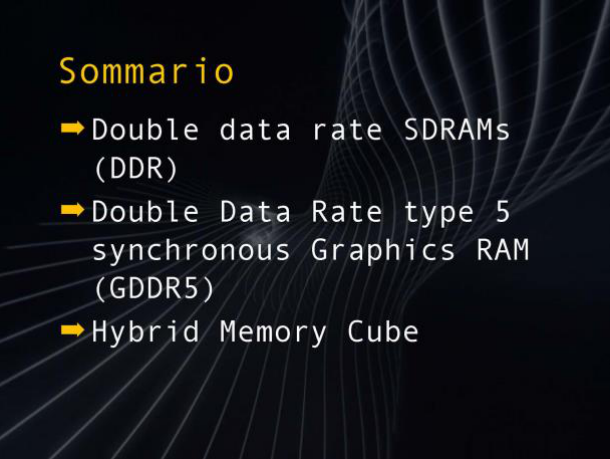
\includegraphics[width=0.40\textwidth,
                    trim=40 80 10 40, % L B R T
                    clip]
                    {images/Lez05_p01_fig_02.png}
  \caption{Sommario}
  \label{fig:Lez05_p01_fig_02}
\end{figure}
\FloatBarrier
\noindent

Il sommario di questa seconda lezione è double data rate SDRAM o DDR in inglese, double data rate type V synchronous graphic RAM o GDDR5 e infine hybrid memory cube che è un nuovo e promettente sistema di memoria.

\section{Double Data Rate Synchronous SDRAM DDR}

Cominciamo con le double data rate synchronous RAM che sono il sistema dominante nel mercato delle memorie dinamiche per architetture di elaborazione.

\FloatBarrier
\begin{figure}[H]
  \centering
  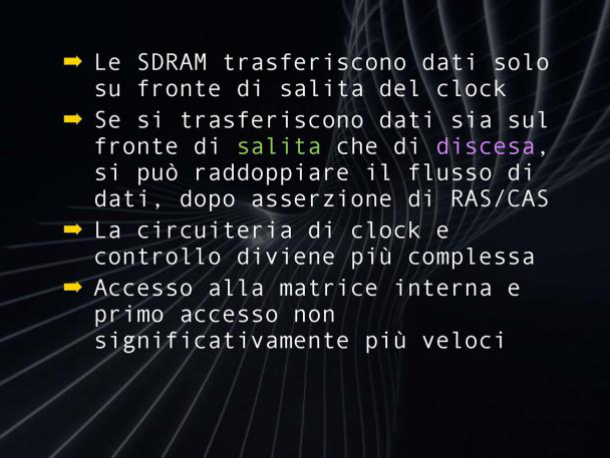
\includegraphics[width=0.40\textwidth,
                    trim=40 80 10 40, % L B R T
                    clip]
                    {images/Lez05_p01_fig_04.png}
  \caption{DDR}
  \label{fig:Lez05_p01_fig_04}
\end{figure}
\FloatBarrier
\noindent

Le SDRAM che abbiamo visto nella lezione precedente trasferiscono dati solo sul fronte di salita del clock.
Quindi la frequenza dei dati che transitano sulle linee di dato ha al massimo una frequenza pari a quella del clock.
Le transizioni al massimo nel caso vi sia una scacchiera bianco nera e pari alla metà di quella del clock.
Immaginate quindi che a una transizione positiva del clock vi sia un dato 1 quindi alto, alla prossima transizione positiva se il dato è ancora 1 non vi è nessuna variazione sulle linee di dato, se al contrario vi è 0 vi è una transizione.
Vi accorgete quindi che il segnale di dati ha una frequenza di segnale pari alla metà di quella del clock, una frequenza informativa pari a quella del clock.
Cercate di non confondere le due differenti frequenze perché questo è un argomento facilmente confondibile.
A parità di piste utilizzate nel circuito stampato ci si accorge quindi che i dati sono più lenti di quello che le caratteristiche elettriche potrebbero permettere e quindi è utile riflettere che se si trasferiscono dati sia sul fronte di salita che di discesa del fronte di clock si può raddoppiaredoppiare il flusso di dati.
Ovviamente questo dopo un'assersione opportuna di RAS e CAS per abilitare l'inizio della lettura o scrittura del processo.

La circuiteria di clock in questo caso diviene un po' più complessa di quella rappresentata già nelle lezioni precedente.

L'accesso alla matrice interna di pass transistors e di trench capacitors al primo accesso non è significativamente più veloce in generale, ma questo è ovviato dal fatto che a parità di tutta l'architettura interna il flusso dei dati sostanzialmente raddoppia per ogni battuta del clock, dell'orologio di sistema. Questo è già un grande vantaggio.

Notate che quello che si fa in questa architettura è sostanzialmente leggere in qualche modo in parallelo due locazioni di memoria, scrivere queste locazioni di memoria in opportuni registri e poi leggere questi registri uno sul fronte positivo e uno sul fronte negativo.
Quindi, contrariamente a quanto avviene nelle normali sdram in cui è letta una locazione, è scritta, poi è letta alla successiva, ovviamente facendo la scansione coi contatori di colonna interna, anche in questo caso si fa coi contatori di colonna interna, però in questo caso vengono accettuti come dire due banchi di memoria in parallelo e questi consentono in questo modo un interallacciamento della lettura su registri e poi i registri vengono letti in sequenza pari, con un ritardo a metà periodo di clock, quindi uno sul fronte positivo e uno sul fronte negativo.

Quindi si riesce ad avere un funzionamento sincrono avendo quindi dati che transitano al doppio della velocità parità di clock e la banda quindi del segnale di dati può essere la stessa della banda del segnale di clock, con un contenuto informativo di due informazioni per periodo di clock.

Questa è importante osservarla, provate quindi nuovamente a fare l'esempio della scacchiera di dati che viene letta o scritta, in questo caso la scacchiera di dati alto-basso-alto-basso sarà sincrona perfettamente al clock, tutt'al più invertita di mezzo pi greco, nel caso sia bianco-nero invece che nero-bianco.

\FloatBarrier
\begin{figure}[H]
  \centering
  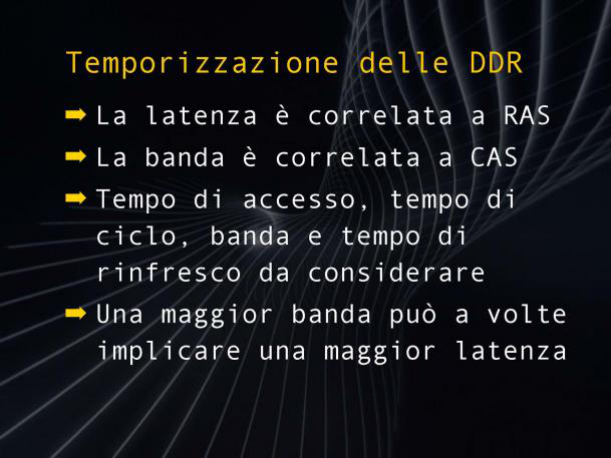
\includegraphics[width=0.40\textwidth,
                    trim=40 80 10 40, % L B R T
                    clip]
                    {images/Lez05_p01_fig_05.png}
  \caption{Temporizzazione DDR}
  \label{fig:Lez05_p01_fig_05}
\end{figure}
\FloatBarrier
\noindent


La temporizzazione delle DDR è una cosa alquanto importante.
Consideriamo che in termini molto semplici ci interessa parlare di latenza, cioè il tempo in cui si accede per primo un dato della memoria, questa in qualche modo è correlata dal tempo che ci mette il row address strobe ad arrivare ed essere raccolto dalla memoria. Quindi questa è la prima risposta che la memoria dà, cioè il row address strobe deve essere comunque lecciato all'interno. Questo ci mette un po' di tempo dipendendo dal tipo di percorsi, soprattutto dalla circuiteria interna e dalla capacità dei circuiti pilota del controllore di asserirlo con una opportuna velocità.

La banda è correlata in generale a column address strobe, cioè con quanta velocità column address strobe riesce ad essere aggiornato internamente, perché vi ripeto che in questo caso si asserisce column address strobe una volta, ma poi viene aggiornato internamente.

Tanto più il contatore di colonna è in grado di scandire rapidamente le locazioni di memoria interne, tanto più sarà elevata la banda in uscita, fermo restando i limiti dettati dagli stati di ingresso e di uscita della memoria e dalle caratteristiche elettriche delle piste che transitano.

In generale dovremo tenere conto di altri parametri, come il tempo di accesso, che ovviamente è la somma di row address strobe e altri parametri, del tempo di ciclo, perché ripeto, ogni volta che si legge una RAM, la RAM deve essere rinfrescata, e questo viene avviata internamente, della banda complessiva del tempo di rinfresco in cui la RAM non può essere utilizzata perché ad esempio viene rinfrescata integralmente.

Notate che in generale una maggior banda può anche implicare una maggior latenza, questo detto così può sembrare banale, ma non è che automaticamente che una memoria che ha una maggior banda, automaticamente diventi anche con minore latenza.
La latenza va quasi in modo indipendente, vi farò vedere fra poco una tabella in cui vi riassume un po' questi parametri per farvi vedere come la banda è aumentata notevolmente negli ultimi anni, ma la latenza non è particolarmente migliorata.

\FloatBarrier
\begin{figure}[H]
  \centering
  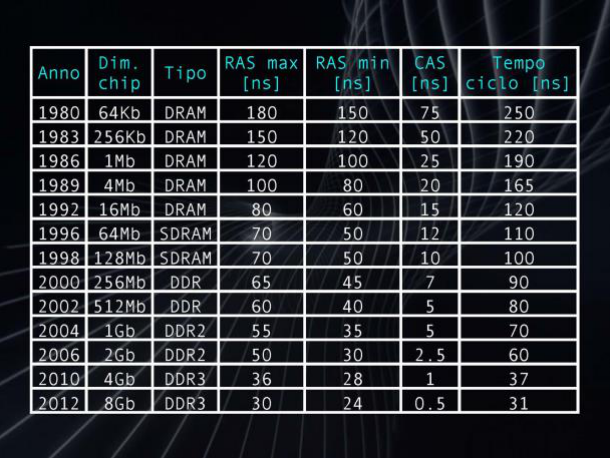
\includegraphics[width=0.70\textwidth,
                    trim=10 30 10 40, % L B R T
                    clip]
                    {images/Lez05_p01_fig_06.png}
  \caption{Confronto nei vari anni}
  \label{fig:Lez05_p01_fig_06}
\end{figure}
\FloatBarrier
\noindent

Vediamo in questa tabella riassuntiva storica che rappresenta circa 35 anni di evoluzione, rappresentiamo l'anno, la dimensione del chip in bit, il bit minuscolo sta per bit, che tipo di RAM è, quindi parliamo qui di DRAM, quindi quando si intende DRAM si intende asincrona, RAS massimo accettabile dal chip, RAS minimo accettabile dal chip, i tempi di CAS, ricordate nell'ultima lezione quando vi faccio vedere le latenze di RAS e CAS, in cui vi avevo fatto vedere un esempio di 3 cicli per RAS e 2 per CAS e poi il tempo di ciclo della memoria, notate che il tempo di ciclo della memoria è maggiore tipicamente della somma, in questo caso è grossomodo pari al massimo RAS più CAS, anche questo è un dato, però significa che non è possibile riaccedere la memoria se non è trascorso almeno questo tempo.
%08:50
Notate come nei passi generazionali legati alla scaling di Moore si è ottenuto, già passando 3 anni, una quadruplicazione della dimensione della RAM, ma i tempi sono diminuiti di poco, in tempo di ciclo complessivo di fatto di poco più di un 10\%.

Passando ancora alla generazione successiva, c'è ancora una quadruplicazione della memoria, in questi anni la legge di Moore veniva utilizzata al suo massimo, quindi lo scaling era molto rapido, i tempi di accesso di RAS e CAS e tempo di ciclo anche qui vedete scalano molto poco; siamo arrivati dopo circa 10 anni ad avere da 64 KB a ben 4 Mb, quindi con un aumento di ben un fattore 64, ma i tempi di ciclo sono diminuiti di circa un terzo rispetto al valore originario, quindi le dimensioni dei chip aumentano notevolmente, i tempi non diminuiscono così rapidamente.

Per tutta la decade degli anni 80 erano asincrone, nella metà degli anni 90 si assiste alle prime SDRAM, in questo caso stiamo parlando di 64 Mb, 8 Mb per chip, i tempi di RAS sono già scesi sotto il centinaio di nanosecondi, notate che però i tempi di RAS fra la generazione precedente del 1992 delle DRAM asincrone e delle SDRAM sincrone a singolo fronte non sono cambiati in maniera significativa, c'è stata una piccola riduzione, in questo caso un 12,5\%, nonostante la banda è aumentata significativamente per il passaggio da una DRAM asincrone alla SDRAM.

I tempi di ciclo sono confrontabili con il valore originario, nonostante tre ordini di grandezza di miglioramento della dimensione, e un miglioramento di un'ordine di grandezza nella velocità di accesso.
Fra una SDRAM e una double data rate nell'arco di due anni il miglioramento è veramente marginale sui tempi di RAS e CAS, forse un pochino più su CAS, ma il tempo di ciclo che è un miglioramento incrementale, ma vi ho già detto la banda era doppia di un fattore 2 fra una SDRAM e una DRAM, quindi banda e latenza non vanno di pari passo.

I miglioramenti tecnologici determinano di fatto un lieve miglioramento di RAS e CAS, ma i circuiti di decodifica interno diventano sempre più grandi e a volte su più livelli, vi ripeto che il fanin e il fanout dei circuiti determina il numero dei livelli. In genere si lavora su fanout di 4 o 5, se si vuole fare un livello di decodifica molto grande e pensate che una RAM da 256 megabit dipendendo da come è organizzata, ad esempio se fosse organizzata su 1 byte, 256 megabit sono 32 megabyte, per indirizzare 32 megabyte servono 25 linee di indirizzo che possono essere divise in 13 linee di riga e 12 di colonna e quindi per decodificare 12 linee non si fa un decoder a 12 ingressi, si fa una gerarchia di decodifica di almeno 2 livelli se non anche 3. Considerate che il numero dei livelli e quindi le latenze interne dei circuiti aumentano all'aumentare della dimensione della memoria per una fissata tecnologia.

Chiaramente la tecnologia migliora, quindi tutti i tempi migliorano, ma non è un aumento così significativo in termini di accesso proprio per questi motivi che vi sto dicendo, cioè della maggior girarchia di decodifica oltre che per il fatto che al diminuire delle dimensioni del disegno, sia dei condensatori che dei transistori, è sempre più difficile far passare una carica da un transistore che è sempre più piccolo perché la sua resistenza aumenta e analogamente è più difficile leggere una carica che è sempre più piccola sui trench capacitors.
Quindi non è facile aumentare la velocità di lettura di una memoria dinamica, al contrario la lettura di una memoria statica può facilmente aumentare ed è aumentata oggettivamente.

Motivo per cui, come vedremo nelle lezioni successive, le cache dei livelli più bassi, cioè le 1 e le 2, sono sempre realizzate in memorie statiche, nonostante siano necessari ben 6 transistori invece di uno solo per ogni bit.

Continuiamo e ci accorgiamo come gli incrementi in tempo sono sempre molto marginali, anche se il CAS, che come vi ho detto determina in qualche modo la banda, è migliorato di oltre un ordine di grandezza nell'arco di 20 anni, RAS non è migliorato sensibilmente, il tempo di ciclo si è ridotto di circa un terzo in 20 anni.

Arriviamo agli anni 2000 con gigabit per chip e le prime DDR2.
Nella sostanza corrisponde a aumentare il livello del prefetch interno, come vi ho detto passare da una SDRAM, una DDR, quello che si fa è si accedono a due locazioni, in una DDR2 si accede a 4 locazioni in contemporanea, ci sono dei buffer interni che registrano questi dati, questi registri vengono letti opportunamente sincronizzati rispetto al clock e quindi pur essendo uguali il tempo di accesso al grande banco di memoria si riescono a leggere utilizzando entrambi i fronti del clock.

Quindi DDR2 hanno un prefetch di 4, un DDR3 ha un prefetch di 8, poi passeremo anche brevemente a accennare le DDR4.
Notate quindi che i tempi sono leggermente migliorati però il tempo di accesso non è neanche scalato di un ordine di grandezza, nonostante il mostruoso incremento della densità delle memorie, quindi memorie sempre più grandi ma non terribilmente più veloci.

\FloatBarrier
\begin{figure}[H]
  \centering
  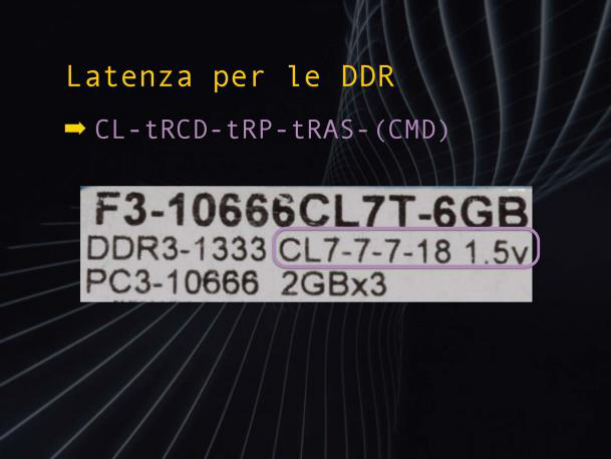
\includegraphics[width=0.50\textwidth,
                    trim=40 40 40 40, % L B R T
                    clip]
                    {images/Lez05_p02_fig_01.png}
  \caption{Esempio di RAM}
  \label{fig:Lez05_p02_fig_01}
\end{figure}
\FloatBarrier
\noindent

Vediamo come si legge un'etichetta di una memoria, in questo caso abbiamo una memoria commerciale in cui ci dice che è una DDR3 1333, 1333 sta per la frequenza in MHz, poi vi sono delle indicazioni che è una PC3 10666, che indica nel modulo la banda in megabyte per secondo, quindi sono 10,666 GB per modulo, poi vediamo qui che si indica 2 GB per 3, quindi questo è un modulo di memoria da 2 GB che viene venduto in una combinazione di tre moduli che possono essere connessi sul bus di sistema su un canale di un processore.
Quindi è possibile montare fino a 3 di questi moduli su 3 slot, cioè su 3 aperture di una scheda madre.
Altri parametri di interesse sono questi individuati qui, CL7-7-7-18 1.5V, 1.5V è la tensione di alimentazione.

\FloatBarrier
\begin{figure}[H]
  \centering
  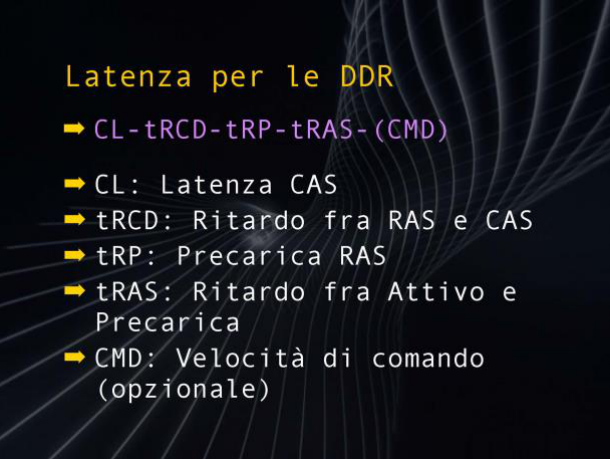
\includegraphics[width=0.50\textwidth,
                    trim=40 40 40 40, % L B R T
                    clip]
                    {images/Lez05_p02_fig_02.png}
  \caption{Caratteristiche}
  \label{fig:Lez05_p02_fig_02}
\end{figure}
\FloatBarrier
\noindent

Questi parametri significano questi acronimi CL, TRCD, TRP, TRaS e CMD.
CL sta per latenza di column address strobe, questo è il tempo quando un comando viene inviato alla memoria e quando la memoria comincia a rispondere, cioè la memoria si accorge di essere stata interpellata solo quando riceve column address strobe. Ci dice in qualche modo quanti cicli delle memoria saranno necessari prima di cominciare a processare il dato.
Notate che tutti questi tempi sono misurati nel clock che arriva alla RAM, che corrisponde alla metà della frequenza che abbiamo visto di 1333.
Non vi ingannate, questo sfortunatamente è un numero sensibilmente più grande.
Nel caso dell'etichetta che abbiamo visto 1333 è quasi 0,8 nanosecondi, però il clock è circa il doppio. Quindi il clock di sistema è di 666 MHz e non di 1333 MHz.
Quindi vanno moltiplicati quei numeri che abbiamo visto tipo 7 per 666, che è circa 1,5 nanosecondi per 7, quindi 10,7 nanosecondi di latenza di CAS.
TRCD è il ritardo fra RAS e CAS.
TRP è il tempo di precarica di RAS, è il numero di cicli che è necessario per poter ricaricare e riattivare una riga, perché, come vi ho detto, appena una riga viene letta, questa deve essere riscritta.
TRAS è il ritardo fra il tempo in cui è attivo e il tempo di precarica e il segnale command dà la velocità di comando in genere è opzionale, questo è un valore che tipicamente è compreso fra 1 e 2 cicli di clock.

Nella targhetta della RAM che vi ho mostrato, command non era indicato perché è un valore quasi sempre fra 1 e 2; quando andate a comprare delle RAM, non vi fate ingannare dai valori di banda, spesso, per certi tipi di applicazione, può anche essere molto più importante la latenza.
Ovviamente la latenza verrà mascherata in buona misura dalla gerarchia di cache, di cui ci occuperemo a partire dalla prossima lezione, però quello che conta in termini di latenza, soprattutto nei casi in cui si accede in modo molto sparso ai dati e le gerarchie di cache risultano meno utili, i tempi di latenza misurati dall'insieme di questi parametri sono quelli che danno il costo di un miss nella gerarchia di cache più alta.

Passeremo a questo argomento nella prossima lezione, però per voi è importante che qualunque scelta di acquisto di progetto non trascuriate di leggere il dato, forse un po' più criptico di queste variabili che vi ho elencate in questa slide, ma sicuramente utile per fare una scelta di progetto, soprattutto in quelle situazioni in cui l'accesso ai dati può avvenire in modo fortemente casuale, non sequenziale a blocchi, perché ogni volta che andate ad accedere alla memoria principale non sarete solo limitati dalla sua banda, ma soprattutto dai tempi di accesso, cioè dalla latenza determinata dall'insieme di questi parametri.

\FloatBarrier
\begin{figure}[H]
  \centering
  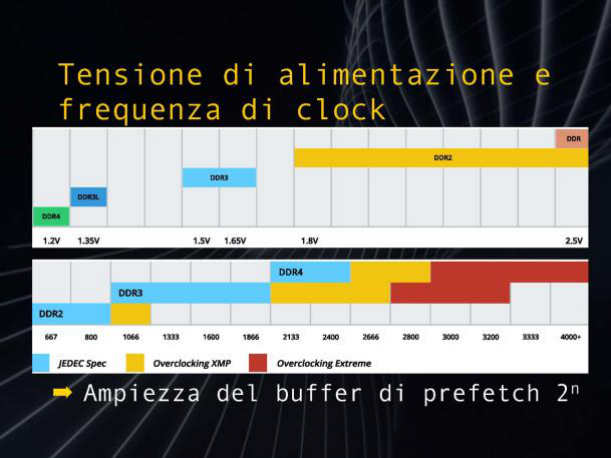
\includegraphics[width=0.50\textwidth,
                    trim=0 40 0 40, % L B R T
                    clip]
                    {images/Lez05_p02_fig_03.png}
  \caption{Caratteristiche}
  \label{fig:Lez05_p02_fig_03}
\end{figure}
\FloatBarrier
\noindent

Vediamo alcuni esempi storici, questo è tratto un po' da una pubblicità di un principale produttore di moduli, vediamo come al variare anche delle generazioni, qui si parte solo dalla DDR, DDR2, DDR3, DDR3 Low Voltage e DDR4.
Vedete come le DDR3 originarie, che abbiamo visto essere metà anni 90, operavano a 2,5 Volt, le DDR2 hanno operato in intervalli compresi fra 1,8 e 2,5, le DDR3 operano fra 1,5 e 1,65, in realtà 1,65 è un po' tirato per le orecchie, quindi il dispositivo scalda e deve essere ben gestita la dissipazione di potenza dal punto vista termico, quindi con dissipatori passivi, cioè radiatori voluminosi, o con ventole, o con dissipazione d'acqua, dove si facciano dei trucchi.
Quali sono i trucchi?
Qualcuno di voi che ama smanettare probabilmente ha provato a fare dell'overclocking della sua scheda madre e del suo processore, a volte anche delle sue RAM, a volte acquistando anche delle RAM certificate per overclocking, questa infatti, come vi ho detto, è la pubblicità di un venditore di moduli che hanno subito, diciamo, una violazione delle specifiche JDEC, l'organismo che standardizza le memorie.
Notate quindi come truccando sulle specifiche nominali, le DDR2 passano da 800 a 1.066 MHz di frequenza di dato, il clock è la metà, come vi ho detto, le DDR3 lavorano nominalmente fra 1.066 e 1.866, ma c'è chi le ha tirate fino a oltre 3 GHz, le DDR3 lavorano nominalmente da 1,866 GHz, le DDR4 già nascono con delle specifiche superiori a 2 GHz e vengono tirate già ad oggi, al momento in cui vi si parla, abbondantemente sopra i 3 GHz.
Notate che questo però spesso viene al costo da un aumento della tensione.
Quindi è importante nella fase di progetto di un sistema di elaborazione tener conto di un insieme di variabili, intanto delle esigenze che avete, è inutile andare più veloce se non ne avete esigenze, spendete più soldi, soprattutto dissipate più energia.
Secondo, la dissipazione della potenza, in questo caso delle DRAM, può essere particolarmente complessa da gestire in un sistema molto compatto, parlo ad esempio dei cosiddetti blade, cioè di quelle architetture di calcolo, generalmente o per server o per calcolo ad alte performance, HPC, high performance computing, in cui si usano delle motherboards con RAM soltanto, senza dischi, dischi sono remoti, in cui sono molto dense per occupare poco spazio e mettere tante motherboard con tanti processori e tante ram.
In quel caso il progetto della dissipazione di potenza può essere critico e se sbagliate il progetto della dissipazione, la prima cosa che fanno, vi friggono le RAM.
In alcuni produttori di questi sistemi infatti utilizzano anche del raffreddamento al liquido e spesso questa potenza è raccolta.
E' un utile esercizio, è utile esercizio anche capire di quanto aumenta la dissipazione di potenza andando a giocare col overclocking, il quale spesso richiede un aumento della tensione e ricordate che la potenza dissipata è $1/2*C*V^2 * f$ f è la frequenza, se aumentate la tensione, aumentate la frequenza, i consumi aumentano.

Nei normali circuiti il consumo aumenta ben più che quadraticamente rispetto alla tensione perché aumentano le correnti di leakage, cioè le correnti di perdite attraverso il transistore.
Quindi state molto cauti quando andate ad aumentare alcuni dei parametri perché il disegno deve essere fatto anche dal punto di vista termico e fotodinamico all'interno del vostro sistema di elaborazione.

Vi riassumo un altro concetto che vi ho detto prima.
L'ampiezza del buffer di lettura delle DDR, DDR2, DDR3, DDR4 cresce sostanzialmente con l'indice N della sigla.
Quindi 2 alla 0, cioè 1 nel caso delle SDRAM, 2 alla 0 nel caso delle DDR, 2 alla 2 nelle DDR2 e così via fino ad arrivare a 2 alla 4 nelle DDR4 che corrisponde a un prefetch buffer di 16.
Quindi ci sono 16 banchi interni che vengono acceduti e questi dati vengono multiplexati verso la lettura in uscita.
Quindi si può andare a un clock molto più veloce ma i tempi interni di scansione di RAS e CAS non diventano particolarmente più veloci come vi ho mostrato nella tabella precedente.

\FloatBarrier
\begin{figure}[H]
  \centering
  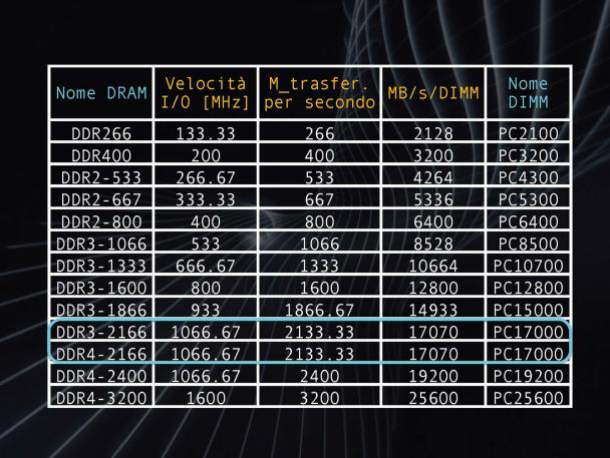
\includegraphics[width=0.60\textwidth,
                    trim=40 40 20 50, % L B R T
                    clip]
                    {images/Lez05_p02_fig_04.png}
  \caption{Caratteristiche}
  \label{fig:Lez05_p02_fig_04}
\end{figure}
\FloatBarrier
\noindent

Qui vediamo un altro riassuntino un po' più sintetico del precedente per porre la vostra attenzione su come leggere le sigle.
Perché il nome delle DRAM che vi ho fatto vedere nella targhetta di quella DRAM rappresenta la velocità dei dati per pin che corrisponde al doppio della frequenza del clock.
Il numero di trasferimenti corrisponde al numeretto che sta dopo la sigla delle DDR.
Il nome della DIMM dà la banda complessiva in megabyte per una DIMM, una Dual In-Line Memory Module, cioè un modulo con connettori da ambole facce, connettori elettrici della schedina, costituita da 64 bit di dato, cioè 8 byte.
Quindi questo numero di megatransfer deve essere moltiplicato per 8 per produrre il throughput, cioè il flusso di dati al secondo per modulo. Il nome del modulo è in genere un arrotondamento del flusso di dati complessivo.
Vediamo adesso un po' rapidamente tutta questa tabella, perché in parte è intuitiva ma vi è utile come riassunto.
Notate però una cosa su cui voglio soffermare la vostra attenzione, è che è possibile a parità di nome del modulo, vedete qui PC 17000, avere sia delle memorie di una generazione che della generazione successiva. Di prima acchito sembrerebbe essere esattamente equivalente dal punto di vista dell'utente. Non sono equivalenti dal punto di vista dei pin, quindi non li potete intercambiare, ma soprattutto non sono equivalenti dal punto di vista della dissipazione, perché abbiamo visto che le DDR4 lavorano a circa 1,2 volt mentre le DDR3 lavorano nominalmente a 1,5, salvo quelle a basso consumo che lavorano a 1,35.
Quindi considerate che la dissipazione potenza è ben significativamente diversa, perché 1,2 al quadrato è molto meno di 1,5 al quadrato.
Vi do uno spunto per la riflessione e vi invito a riflettere come si potrebbe ulteriormente incrementare la velocità rispetto al funzionamento a doppio fronte del clock.

Sfortunatamente la risposta è non facciamo quattro fronti, quattro transizioni, perché non è così banale a farsi.
In realtà in parte è vero, in parte non è vero quello che vi ho detto in questo termine, perché è facile fare un sincronismo sul fronte positivo e sul fronte negativo. 
Trasferire più dati rispetto ai fronti richiede una certa cura dal punto di vista della stabilità dei sistemi elettrici, delle connessioni e a volte anche l'estrazione di un sincronismo da un dato che deve rimanere molto stabile.
In linea di principio è possibile trasferire il contenuto informativo dei dati con una frequenza maggiore di quella del clock, ma si richiede particolare attenzione. Esistono però delle situazioni in cui questo si rivela necessario.

\subsection{GDDR5 }

Il caso particolare è quello delle memorie per schede grafiche, cioè acceleratori grafici o processori grafici.
Sono state quindi introdotte le cosiddette Double Data Rate Type 5 Synchronous Graphic RAM, in gergo GDDR5.

\FloatBarrier
\begin{figure}[H]
  \centering
  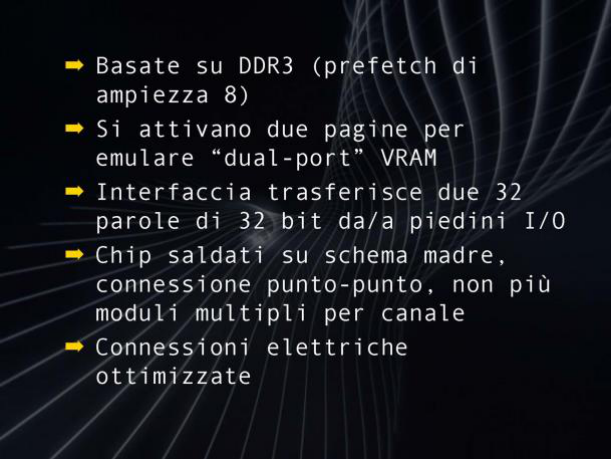
\includegraphics[width=0.50\textwidth,
                    trim=40 40 40 40, % L B R T
                    clip]
                    {images/Lez05_p03_fig_01.png}
  \caption{Caratteristiche}
  \label{fig:Lez05_p03_fig_01}
\end{figure}
\FloatBarrier
\noindent

Queste sono basate sostanzialmente sulle DDR3, che sono con un prefetch buffer di 8.
Notate che il numero 5 è solamente pubblicitario, ma di fatto internamente sono in buona parte basate sul principio delle DDR3, che è quello della larghezza del prefetch buffer.
Una caratteristica peculiare è quella che si attivano due pagine per emulare le cosiddette memorie a doppia porta, Dual Port, delle video RAM. Perché questo è necessario? Perché spesso è necessario fare una scansione della memoria per rappresentare su uno schermo l'informazione e allo stesso tempo scrivere l'informazione nuova come è stata processata dal processore grafico.
In passato si usavano due porte diverse, una di scrittura e una di lettura. Questo può essere fatto velocemente con una sola porta, dove però sono attive contemporaneamente delle pagine diverse per poter più rapidamente gestire gli aggiornamenti.
Richiede chiaramente un po' più di circuteria.

La caratteristica delle DDR è un'interfaccia che trasferisce due parole di 32 bit da/a piedini, quindi tutta la memoria è fatta da multipli di 2x32 bit.
I chip sono sempre saldati su scheda madre, la connessione è punto punto e non vi sono più moduli multipli per canale, come abbiamo visto ad esempio nel caso della targhetta precedente dove tre moduli erano possibili per una DDR3.

Nel caso delle GDDR5 in nessun modo è possibile attaccare moduli, tanto meno attaccare più di un modulo.
Per avere una buona caratteristica dei segnali elettrici è necessario saldare quanto più vicino al processore video, in questo caso, i chip e stare anche molto attenti alla qualità delle piste elettriche.
Infatti le condizioni elettriche devono essere ottimizzate e ben studiate per evitare differenze dei percorsi di cui vi ho detto ad esempio una curva.

\FloatBarrier
\begin{figure}[H]
  \centering
  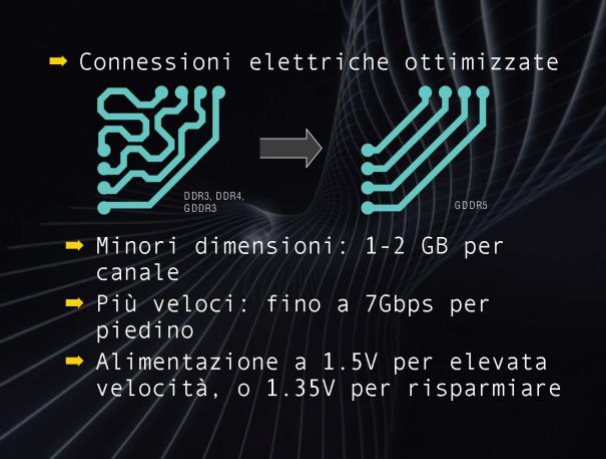
\includegraphics[width=0.50\textwidth,
                    trim=40 40 40 40, % L B R T
                    clip]
                    {images/Lez05_p03_fig_02.png}
  \caption{Caratteristiche}
  \label{fig:Lez05_p03_fig_02}
\end{figure}
\FloatBarrier
\noindent

È anche importante quindi ottimizzare le caratteristiche, ad esempio non si realizzano dei circuiti fatti da un routing automatico di un software pensato ad Orchard ma le piste devono essere realizzate in questo modo e anche in questo caso la differente lunghezza determina un differente ritardo e deve essere opportunamente tenuto in conto.
In generale andare veloci impone sempre minori dimensioni, tipicamente ci sono 1 o 2 GB per canale, contro a volte i 96 GB delle DDR3, anche se un po' costose, sono però molto più veloci, si possono avere fino a 7 GB per secondo per piedino.
Abbiamo visto nella slide pubblicitaria precedente delle RAM overclockate, le DDR3 arrivano tirandole fuori specifica attorno ai 3 GB, le DDR4 attorno a 4 GB per piedino.
Le GDDR5 consentono bande di un paio di volte superiore, sono già disponibili commercialmente senza violare alcuna specifica.
L'alimentazione lavora tipicamente a 1,5 V come le DDR3, visto che da esse derivano, ma è anche possibile mettere una modalità diciamo basso consumo da 1,35.
Immaginate di dover giocare col vostro videogioco e lì avete bisogno il massimo delle performance, invece pensate a un word processor tipo un editor in cui la quantità di dati è ben poca da aggiornare e si può anche ridurre la tensione e quindi anche ridurre eventualmente la frequenza di scansione delle stesse.

\FloatBarrier
\begin{figure}[H]
  \centering
  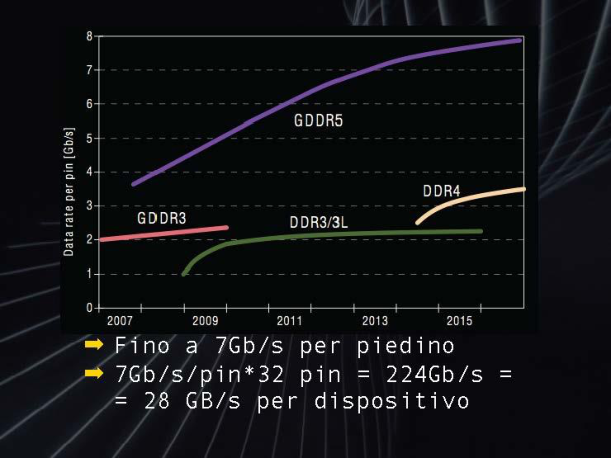
\includegraphics[width=0.50\textwidth,
                    trim=40 40 40 10, % L B R T
                    clip]
                    {images/Lez05_p03_fig_03.png}
  \caption{Caratteristiche}
  \label{fig:Lez05_p03_fig_03}
\end{figure}
\FloatBarrier
\noindent

Qui vi faccio vedere un grafico che vi rappresenta la differenza anche in termini evolutivi delle diverse generazioni di DDR4, DDR3 che abbiamo visto prima, queste sono all'interno delle specifiche nominali, quindi si arriva a 2,133 GB per le DDR3, non alle versioni overclockate.
Le GDDR3 erano la generazione precedente delle GDDR5, non c'è mai stata una 4, diciamo che la pubblicità e il marketing fa la sua parte nel mettere dei numeri più grandi, ma questa tecnologia corrisponde a questa tecnologia.
Come ho detto fino a 7 GB per piedino, considerando 7 GB secondo per pin per 32 pin ci sono 224 GB per secondo pari a 28 GB per dispositivo.

\FloatBarrier
\begin{figure}[H]
  \centering
  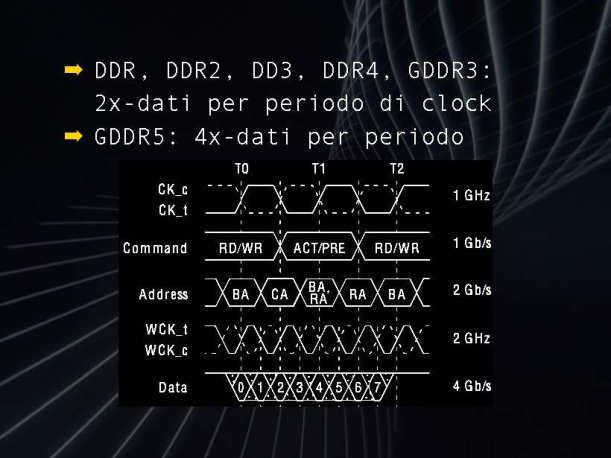
\includegraphics[width=0.50\textwidth,
                    trim=40 40 40 10, % L B R T
                    clip]
                    {images/Lez05_p03_fig_05.png}
  \caption{Caratteristiche}
  \label{fig:Lez05_p03_fig_05}
\end{figure}
\FloatBarrier
\noindent

Vediamo quindi che nel caso delle DDR, DDR2, DDR3, DDR4 e anche le precedenti GDDR3 ci sono due dati per periodo di clock, al contrario nelle GDDR5 sono ben 4 dati per periodo di clock, come viene fatto questo?
Vi faccio qui rapidamente vedere i sincronismi, ma quello che succede è che i dati commudono più rapidamente del clock, quindi è molto importante che internamente i segnali siano ben fatti e cosa avviene?
Per ogni blocco di 2 byte che non vi mostrerò, vi sono due clock differenziali, vedete quindi due linee di clock sfasate di mezzo periodo, in maniera tale da dare quindi il doppio livello di sincronismo, quindi si raddoppiano le linee di clock per raddoppiare la banda rispetto alla frequenza di clock.

\FloatBarrier
\begin{figure}[H]
  \centering
  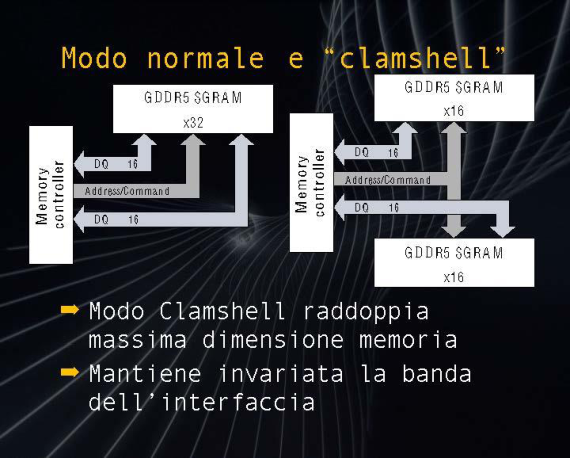
\includegraphics[width=0.50\textwidth,
                    trim=20 20 20 20, % L B R T
                    clip]
                    {images/Lez05_p03_fig_06.png}
  \caption{Caratteristiche}
  \label{fig:Lez05_p03_fig_06}
\end{figure}
\FloatBarrier
\noindent

Un modo per utilizzare le GDDR è anche questo, c'è un chip GDDR, vi ho detto, da 32 bit, due linee da 16 bit, ognuno di questi con un doppio clock che non vi mostro ma vi lascerò nelle slide, e le piste di indirizzo.
Se vogliamo raddoppiare la quantità di memoria si usa la cosiddetta modalità Clamshell, cioè a conchiglia bivalva, in cui si utilizzano le stesse linee di indirizzo, in questo caso si multiplexa connesse in parallelo, ma i dati rimangono ognuno di loro, ognuno del blocco di 16 bit, cioè due canali da qua da 8 bit, separati.
In questo modo si raddoppia la massima dimensione della memoria ma si mantiene invariata la banda dell'interfaccia, che è sempre quella 32 per la frequenza massima, come abbiamo visto per esempio nell'esempio precedente.
Ad esempio con un bus a 256 bit, cioè 8 interface da 32 e chip da 2 gigabit, si ottengono 2 gigabyte con 8 chip nella modalità normale per 32 o 4 gigabyte con 8 chip in modalità per 16.

Quindi vi do uno spunto per la riflessione e vi invito a riflettere come si potrebbe ulteriormente incrementare sia la velocità e allo stesso tempo anche avere dimensioni maggiori che delle GDDR5.

Abbiamo detto che non li possiamo mettere in parallelo ma possiamo fare un'altra cosa, possiamo ancora di più giocare sulla configurazione e l'impacchettamento della memoria.

\subsection{Hybrid Memory Cuba}

Quindi abbiamo in questo modo una potenzialmente futura architettura di memoria, le cosiddette hybrid memory cube, che ancora non sono in vendita ma sono ampiamente standardizzate dai principali produttori.

\FloatBarrier
\begin{figure}[H]
  \centering
  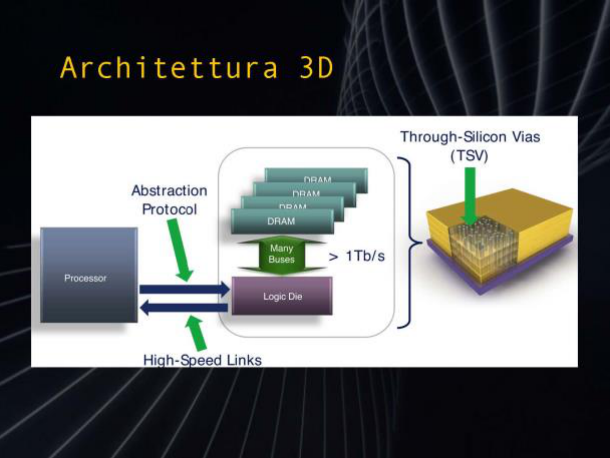
\includegraphics[width=0.50\textwidth,
                    trim=20 80 20 20, % L B R T
                    clip]
                    {images/Lez05_p04_fig_04.png}
  \caption{Caratteristiche}
  \label{fig:Lez05_p04_fig_04}
\end{figure}
\FloatBarrier
\noindent

La logica qual è? Invece di avere chip su moduli come i DIMM del GDDR e GDDR4 o saldate su board, si saldano chip su chip attraverso quelli che si chiamano true silicon bias, cioè dei passaggi.
Quindi queste sono proprio i singoli chip di silicio sovrapposti, ad esempio 8, montate su un altro chip che contiene un po' di logica, quindi logica di decodifica, ma le varie moduli delle DRAM dense sono sovrapposte l'una all'altra.

\FloatBarrier
\begin{figure}[H]
  \centering
  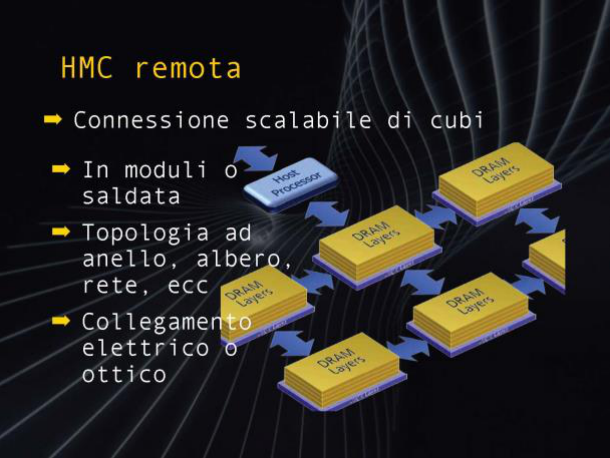
\includegraphics[width=0.50\textwidth,
                    trim=20 20 20 20, % L B R T
                    clip]
                    {images/Lez05_p04_fig_05.png}
  \caption{Caratteristiche}
  \label{fig:Lez05_p04_fig_05}
\end{figure}
\FloatBarrier
\noindent

Quindi sono tutti questi moduli messi in questo modo, si può arrivare a 1 Tbps per connessione, possono essere utilizzati all'interno del package in una architettura multi-chip package, quindi immaginate come una girarchia ad esempio di cache veloci o le RAM video dell'acceleratore grafico, questo consente la massima dimensione di banda perché si utilizzano minime distanze, quindi i segnali possono essere più veloci.

\FloatBarrier
\begin{figure}[H]
  \centering
  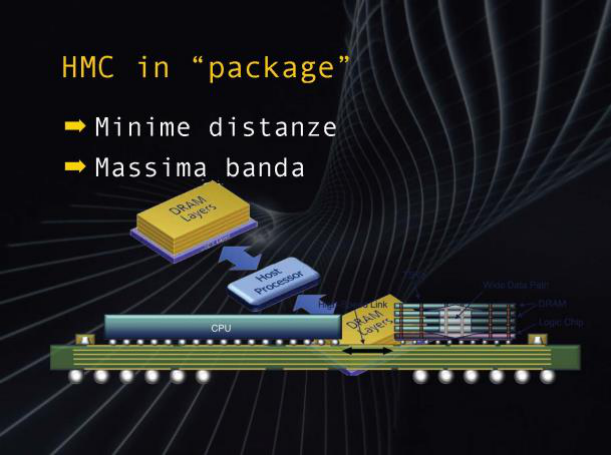
\includegraphics[width=0.50\textwidth,
                    trim=20 20 20 20, % L B R T
                    clip]
                    {images/Lez05_p04_fig_06.png}
  \caption{Caratteristiche}
  \label{fig:Lez05_p04_fig_06}
\end{figure}
\FloatBarrier
\noindent

Oppure dal punto di vista architetturale c'è quindi una daughterboard o un package multilayer, a volte ceramico, a volte polimerico, in cui c'è un microprocessore saldato in ball grid array, cioè array di palline, e qua sopra lo stack, cioè la sovrapposizione in questo caso di 4 moduli di DIMM con un chip logico disegnato qui in colore viola diverso dal colore dei chip stessi.
Questo consente la massima velocità perché si minimizano i percorsi.
Oppure utilizzata come viene attualmente utilizzata una normale FB DIMM dove ci sono tanti modulini sovrapposti stacked ancora interconnessi in qualche modo scalabile, ad esempio qui in una mesh, ma i moduli possono essere o saldati o messi su moduli disgiunti, si può creare una topologia ad albero, a rete, in questo caso a rete o ad anello, a seconda delle scelte, perché ognuno dei moduli logici hanno dei canali, ad esempio in questo caso ne sono rappresentati 4, per realizzare una mesh.
Addirittura questi possono avere dei moduli ottici per poter quindi anche ridurre il problema dei parassiti che affliggono le linee elettriche.
